\documentclass{article}
\usepackage[utf8]{inputenc}
\usepackage[english]{babel}
\usepackage [autostyle, english = american]{csquotes}
\MakeOuterQuote{"}
\usepackage{graphicx}
\usepackage{enumerate}
\usepackage{float}
\graphicspath{ {} }
\usepackage{mathtools}
\usepackage{amsmath, amsthm, amssymb, amsfonts}
\usepackage{caption}
\usepackage{bm}
\usepackage{fancyhdr}
\pagestyle{fancy}
\fancyhf{}
\rhead{Ty Darnell}
\lhead{Homework 11}

% For derivatives
\newcommand{\deriv}[1]{\frac{\mathrm{d}}{\mathrm{d}x} (#1)}

% For partial derivatives
\newcommand{\pderiv}[2]{\frac{\partial #1}{\partial #2}}

% Integral dx
\newcommand{\dx}{\mathrm{d}x}
\newcommand{\cd}{\overset{d}{\to}}
\newcommand{\cp}{\overset{p}{\to}}
\newcommand{\B}{\beta}
\newcommand{\e}{\epsilon}
\newcommand{\limn}{\lim_{n\to \infty}}
\newcommand{\lm}{\lambda}
\newcommand{\sg}{\sigma}
\newcommand{\hb}{\hat{\beta}}
\newcommand{\sumn}{\sum_{i=1}^{n}}
\newcommand{\hth}{\hat{\theta}}
\newcommand{\lra}{\Leftrightarrow}
\newcommand{\prodn}{\prod_{i=1}^{n}}
\newcommand{\dll}[1]{\dfrac{\partial\ell}{\partial{#1}}}
\newcommand{\mle}{\hat{\theta}_{MLE}}
\newcommand{\mm}{\hat{\theta}_{MM}}
\newcommand{\sumx}{\sum_{i=1}^{n}x_i}
\newcommand{\ta}{\theta}
\newcommand{\qe}{ \ ?\ }
\newcommand{\dt}{\pderiv{}{\ta}}
\newcommand{\lt}[1]{\log(f(#1|\ta))}
\newcommand{\lx}{\lambda(x)}
\newcommand{\samp}{X_1,\dots,X_n \sim}
\newcommand{\te}{\theta_1}
\newcommand{\xm}{x_{(1)}}
\newcommand{\Xn}{X_{(n)}}
\newcommand{\sn}{(\sg^2)}
\newcommand{\pow}{\B(\ta)}
\newcommand{\hyp}[2]{H_0: #1 \text{ vs } H_1: #2}
\newcommand{\pois}[2]{\dfrac{e^{-#1}{#1}^{#2}}{{#2}!}}
\newcommand{\mlr}{\dfrac{f(x|\ta_2)}{f(x|\ta_1)}}
\newcommand{\al}{\alpha}
\newcommand{\bx}{\bar{x}}
\newcommand{\by}{\bar{y}}
\newcommand{\Bx}{\bar{X}}
\newcommand{\By}{\bar{Y}}
\newcommand{\sx}{\sg_X^2}
\newcommand{\sy}{\sg_Y^2}
\newcommand{\so}{\sg_0^2}
\newcommand{\lo}{\lm_0}
\allowdisplaybreaks
\begin{document}
\begin{flushleft}

\section*{Problem 1}
\begin{enumerate}[(a)]
	
	\item 
\begin{multline*}\\
X_1,\dots,X_n \sim
P(X_i\leq x|\alpha,\B)=\begin{cases}
0  & x<0\\
(x/\B)^{\alpha}  & 0\leq x\leq\B\\
1  & x>\B
\end{cases}\\
\al, \ \B \text{ are positive}\\
\hat{\B}_{MLE}=X_{(n)} \text{ (from problem 7.10)}\\
\al=\al_0\\
\text{Pivot}=X_{(n)} /\B\\
.05=P(X_{(n)}/\B\leq c)=P(X_1,\dots,X_n\leq c\B)=\left(\dfrac{c\B}{\B}\right)^{\al_0n}=c^{\al_0n}\\
.05^{1/(\al_0n)}=c\\
.95=P(\Xn/\B>c)=P(\Xn/c>\B)\\
=P(\Xn/.05^{1/(\al_0n)}>\B)\\
\{\B:\B< \Xn/(.05^{1/(\al_0n)})\}\\
\end{multline*}

	\item 
\begin{multline*}\\
\hb_{MLE}=\Xn=25\\
\hat{\al}_{MLE}=12.59 \quad n=14\\
\{\B:\B< 25/(.05^{1/(12.59*14)})\}\\
25/(.05^{1/(12.59*14)})=25.42853=25.43\\
\B<25.43\\
\text{Since } \B \text{ is positive, the lower bound cannot be below 0}\\
\text{Thus the interval for } \B \text{ is } (0,25.43)\\
\end{multline*}

\end{enumerate}
\pagebreak
	\section*{Problem 2}
\begin{enumerate}[(a)]
	
	\item 
\begin{multline*}\\
\samp N(0,\sg^2_X) \quad Y_1,\dots,Y_m \sim N(0,\sg^2_Y) \quad X\perp Y\\
\lm=\sg^2_Y/\sg^2_X\\
\hyp{\lm=\lm_0}{\lm \neq \lm_0}\\
\lm(x,y)=\dfrac{\sup_{\lm=\lm_0}L(\sg^2_X,\sg^2_Y|x,y)}{\sup_{\lm \in \Theta}L(\sg^2_X,\sg^2_Y|x,y)}\\
\text{Unrestricted MLEs:}\\
\hat{\sg^2_X}_{MLE}=\sumn X_i^2/n \quad \hat{\sg^2_Y}_{MLE}=\sumn Y^2_i/m\\
L(\sx,\sy|x,y)=(2\pi)^{-(n+m)/2}( \sx)^{-n/2}( \sy)^{-m/2}\exp\left(-\sum x_i^2/(2\sx) \right)\exp\left(-\sum y_i^2/(2\sy) \right)\\
\text{Under } H_0: \quad \lm=\lm_0=\sg^2_Y/\sg^2_X\\
\sg^2_Y=\lm_0 \sg_X^2\\
L(\sx,\lm_0\sy|x,y)=(2\pi\sx)^{-n/2}(2\pi \lo\sx)^{-m/2}\exp\left(-\sum x_i^2/(2\sx) \right)\exp\left(-\sum y_i^2/(2\lo\sx) \right)\\
=(2\pi)^{-(n+m)/2}(\sx)^{-(n+m)/2}\lo^{-m/2}\exp\left(-\left[\lo\sum x_i^2+\sum y_i^2\right]/(2\lo \sx)\right)\\
\ell=-((n+m)/2)\log(2\pi) -((n+m)/2)\log(\sx)-(m/2)\log(\lo)-\left[\lo\sum x_i^2+\sum y_i^2\right]/(2\lo \sx)\\
\dll{\sx}=-\dfrac{(n+m)/2}{\sx}+\dfrac{\lo\sum x_i^2+\sum y_i^2}{2\lo(\sx)^2 }=0\\
\dfrac{(n+m)/2}{\sx}=\dfrac{\lo\sum x_i^2+\sum y_i^2}{2\lo(\sx)^2 }\\
\hat{\sg^2_0}=\dfrac{\lo\sum x_i^2+\sum y_i^2}{\lo(n+m)}\\
\pderiv{\ell^2}{(\sx)^2}=\dfrac{(n+m)/2}{(\sx)^2}-\dfrac{\lo\sum x_i^2+\sum y_i^2}{\lo(\sx)^3 }\\
\text{Plugging in } \hat{\so}:\\
=\left(\dfrac{\lo(n+m)}{\lo\sum x_i^2+\sum y_i^2}\right)^2\left[(n+m)/2-\dfrac{\lo\sum x_i^2+\sum y_i^2}{\lo}\dfrac{\lo(n+m)}{\lo\sum x_i^2+\sum y_i^2}\right]\\
=\left(\dfrac{\lo(n+m)}{\lo\sum x_i^2+\sum y_i^2}\right)^2(-(n+m)/2)\\
=-\dfrac{(\so)^2(n+m)}{2}<0\\
\text{Thus } \hat{\so} \text{ is the MLE}\\
\lm(x,y)=\dfrac{(\hat{\so})^{-(n+m)/2}\lo^{-m/2}\exp\left(-\left[\lo\sum x_i^2+\sum y_i^2\right]/(2\lo \hat{\so})\right)}{( \hat{\sx})^{-n/2}( \hat{\sy})^{-m/2}\exp\left(-\sum x_i^2/(2\hat{\sx)}-\sum y_i^2/(2\hat{\sy}) \right)}\\
=\dfrac{( \hat{\sx})^{n/2}( \hat{\sy})^{m/2}\exp\left(-\left[\lo\sum x_i^2+\sum y_i^2\right]/(2\lo \hat{\so})+\sum x_i^2/(2\hat{\sx})+\sum y_i^2/(2\hat{\sy}) \right)}{(\hat{\so})^{(n+m)/2}\lo^{m/2}}\\
=\dfrac{( \hat{\sx})^{n/2}( \hat{\sy})^{m/2}\exp\left(-(n+m)/2+(n/2)+(m/2) \right)}{(\hat{\so})^{(n+m)/2}\lo^{m/2}}\\
\lm(x,y)=\dfrac{( \hat{\sx})^{n/2}( \hat{\sy})^{m/2}}{(\hat{\so})^{(n+m)/2}\lo^{m/2}}\\
R=\{(x,y):\lm(x,y)<c \} \text{ Where c is chosen to give the test size } \al\\
\end{multline*}

	\item 
\begin{multline*}\\
\text{Under } H_0: \ \lo=\lm=\sy/\sx\\
\text{Let } A=\sum Y_i^2/(\lo\sx)=\sum Y_i^2/\sy \sim \chi^2_m\\
\text{Let } B=\sum X_i^2/\sx\sim \chi^2_n\\
A\perp B\\
\text{Let } F=\dfrac{A}{B}\dfrac{n}{m}=\dfrac{(\sum Y_i^2/\sy)/m}{(\sum X_i^2/\sx)/ n}=\dfrac{\sum Y_i^2/(\lo m)}{\sum X_i^2/n}\sim F_{m,n}\\
\lm(x,y)=\left( \dfrac{\hat{\sx}}{\hat{\so}}\right)^{n/2}\left( \dfrac{\hat{\sy}}{\hat{\so} \lo}\right)^{m/2} \\
 \dfrac{\hat{\sx}}{\hat{\so}}=\dfrac{n+m}{n}\dfrac{\sum X_i^2 \lo}{\lo \sum X_i^2+\sum Y_i^2}\\
=\dfrac{n+m}{n}\dfrac{\sum X_i^2 \lo}{\lo \sum X_i^2+\sum Y_i^2}\\
=\dfrac{n+m}{n}\dfrac{1}{1+(\sum Y_i^2/ \sy)/(\sum X_i^2/\sx)}\\
=\dfrac{n+m}{n+nA/B}\\
=1/\left(\dfrac{n+nA/B}{n+m}\right)\\
=1/\left(\dfrac{n}{n+m}+\dfrac{1}{m+n}\dfrac{mnA}{mB}\right)\\
=1/\left(\dfrac{n}{n+m}+\dfrac{m}{m+n}F\right)\\
\dfrac{\hat{\sy}}{\hat{\so} \lo}=\dfrac{n+m}{m}\dfrac{\sum Y_i^2}{\lo \sum X_i^2+\sum Y_i^2}\\
\dfrac{n+m}{m}\dfrac{1}{1+(\sy \sum X_i^2)/(\sum Y_i^2\sx)}\\
=1/\left(\dfrac{m}{n+m}\left[1+\dfrac{\sy \sum X_i^2}{\sx \sum Y_i^2}\right]\right)\\
=1/\left(\dfrac{m}{n+m}(1+B/A)\right)\\
=1/\left(\dfrac{m}{n+m}+\dfrac{1}{n+m}\dfrac{mB}{A}\dfrac{n}{n}\right)\\
=1/\left(\dfrac{m}{n+m}+\dfrac{n}{n+m}\dfrac{mB}{nA}\right)\\
=1/\left(\dfrac{m}{n+m}+\dfrac{n}{n+m}F^{-1}\right)\\
\lm(x,y)=\left(\dfrac{1}{\dfrac{n}{n+m}+\dfrac{m}{m+n}F}\right)^{n/2}\left(\dfrac{1}{\dfrac{m}{n+m}+\dfrac{n}{n+m}F^{-1}}\right)^{m/2}\\
R=\left\{(x,y):\left(\dfrac{1}{\dfrac{n}{n+m}+\dfrac{m}{m+n}F}\right)^{n/2}\left(\dfrac{1}{\dfrac{m}{n+m}+\dfrac{n}{n+m}F^{-1}}\right)^{m/2}<c_\alpha \right\}\\
\text{Where } c_\al \text{ satisfies:}\\
P\left(\left(\dfrac{1}{\dfrac{n}{n+m}+\dfrac{m}{m+n}F}\right)^{n/2}\left(\dfrac{1}{\dfrac{m}{n+m}+\dfrac{n}{n+m}F^{-1}}\right)^{m/2}<c_\alpha\right)=\al\\
\end{multline*}
	\item 
\begin{multline*}\\
\lm(x,y)=\left(\dfrac{n}{n+m}+\dfrac{m}{n+m}\dfrac{\sum Y_i^2}{\sum X_i^2\lm}\dfrac{n}{m}\right)^{-n/2} \left(\dfrac{m}{n+m}+\dfrac{n}{n+m}\dfrac{\sum X_i^2\lm}{\sum Y_i^2}\dfrac{m}{n}\right)^{-m/2}\\
=\left(\dfrac{n}{n+m}+\dfrac{n}{n+m}\dfrac{\sum Y_i^2}{\sum X_i^2\lm}\right)^{-n/2} \left(\dfrac{m}{n+m}+\dfrac{m}{n+m}\dfrac{\sum X_i^2\lm}{\sum Y_i^2}\right)^{-m/2}\\
\text{Let } D=\dfrac{n}{n+m} \text{ and } E=D\dfrac{\sum Y_i^2}{\sum X_i^2}=\dfrac{n}{n+m}\dfrac{\sum Y_i^2}{\sum X_i^2}\\
\lm(x,y)=\left(D+\dfrac{E}{\lm}\right)^{-n/2}\left((1-D)+(1-D)\dfrac{D\sum Y_i^2}{D\sum X_i^2}\lm\right)^{-m/2}\\
\lm(x,y)=\left(D+\dfrac{E}{\lm}\right)^{-n/2}\left((1-D)+(1-D)D\dfrac{\lm}{E}\right)^{-m/2}\\
\text{The acceptance region is:}\\
A=\left\{\lm(x,y):\left(D+\dfrac{E}{\lm}\right)^{-n/2}\left((1-D)+(1-D)D\dfrac{\lm}{E}\right)^{-m/2}\geq c_a\right\}\\
\text{Inverting the acceptance region we have the } 1-\al \text{ CI for } \lm:\\
C(\lm)=\left\{\lm:\left(D+\dfrac{E}{\lm}\right)^{-n/2}\left((1-D)+(1-D)D\dfrac{\lm}{E}\right)^{-m/2}\geq c_a\right\}\\
\text{Multiplying both sides by } \left(\dfrac{E}{1-D}\right)^{-m/2} \text{ we have:}\\
\left(D+\dfrac{E}{\lm}\right)^{-n/2}\left([(1-D)+(1-D)D\dfrac{\lm}{E}]\left(\dfrac{E}{1-D}\right)\right)^{-m/2}\geq c_a\left(\dfrac{E}{1-D}\right)^{-m/2}\\
\left(D+\dfrac{E}{\lm}\right)^{-n/2}\left(E+D\lm\right)^{-m/2}\geq c_a\left(\dfrac{E}{1-D}\right)^{-m/2}\\
\text{taking the derivative of the log with respect to } \lm \text{ of the left side:}\\
\pderiv{}{\lm}(-n/2)\log(D+E/\lm)-(m/2)\log(E+D\lm)\\
=\dfrac{nE-mD\lm}{2\lm(E+D\lm)}\Rightarrow(1/2)\dfrac{n\dfrac{n}{n+m}\dfrac{\sum Y_i}{\sum X_i}-m\dfrac{n}{n+m}\lm}{\lm(\dfrac{n}{n+m}\dfrac{\sum Y_i}{\sum X_i}+\dfrac{n}{n+m}\lm)}\\
\text{Let } S=\dfrac{\sum Y_i}{\sum X_i}\\
=(1/2)\dfrac{nS-m\lm}{\lm(S+\lm)}\Rightarrow
(1/2)\dfrac{nS/\lm-m}{S+\lm}\\
\text{For } \lm\geq 0 \text{ the derivative} \text{ changes sign from positive to negative,}\\
\text{thus } C(\lm) \text{ increases and decreases and is therefore an interval}\\
\text{The graph of } C(\lm) \text{ is a parabola}\\
\end{multline*}
	
\end{enumerate}

	\section*{Problem 3}
	
\begin{enumerate}[(a)]
	\item 
\begin{multline*}\\
\samp f(x|\ta)=1, \quad \ta-1/2<x<\ta+1/2\\
Y=X-\ta \\
f_Y(y)=1 \quad -1/2<y<1/2 \quad Y\perp \ta\\
Y\sim U(-1/2,1/2)\\
1-\al=P(\al_1-1/2\leq X-\ta\leq 1/2-\al_2)\\
1-\al=P(X_1-(1/2-\al_2)\leq\ta\leq X_1-(\al_1-1/2))\\
1-\al \text{ CI}=(\al_2-1/2,1/2-\al_1)\\
\end{multline*}
	
	\item 
\begin{multline*}\\
\samp f(x|\ta)=2x/\ta^2, \quad 0<x<\ta, \ \ta>0\\
Y=X/\ta \quad \dfrac{dy}{dx}=1/\ta\\
f_y(y)=f_x(\ta y)=\dfrac{1}{|1/\ta|}=\dfrac{2y\ta}{\ta^2}\ta\\ 
f_Y(y)=2y \quad 0\leq y\leq 1 \quad Y\perp \ta\\ 
P(a\leq X/\ta\leq b)=\int_{a}^{b}2y \ dy=b^2-a^2\\
b^2-a^2=1-\al \Rightarrow b^2-a^2=\sqrt{1-\al/2}^2-\sqrt{\al/2}^2\\
b=\sqrt{1-\al/2} \quad a=\sqrt{\al/2}\\
\end{multline*}

	
\end{enumerate}

	\section*{Problem 4}
	
\begin{enumerate}[(a)]
	
	\item 	
\begin{multline*}\\
\samp f(x|\ta)=(a/\ta)(x/\ta)^{a-1} \quad 0<x<\ta\\
CDF\sim U(0,1)\\
1-\alpha=P(\al_1<F_{\Xn}(x)<1-\al_2)\\
F_{\Xn}(x)=P(\Xn\leq x)=[P(X_1\leq x)]^n\\
P(X_1\leq x)=\int_{0}^{x}(a/\ta)(y/\ta)^{a-1}\ dy=(x/\ta)^{a}\\
[P(X_1\leq x)]^n=(x/\ta)^{an}\\
1-\al=P(\al_1<(\Xn/\ta)^{an}<1-\al_2)\\
=P(\al_1^{1/(an)}<\Xn/\ta<(1-\al_2)^{1/(an)})\\
=P(\Xn/(1-\al_2)^{1/(an)}<\ta<\Xn/\al_1^{1/(an)})\\
1-\al \text{ CI }= \left(\dfrac{\Xn}{(1-\al_2)^{1/(an)}},\dfrac{\Xn}{\al_1^{1/(an)}} \right)\\
\end{multline*}

	\item 
\begin{multline*}\\
Y=\left(\dfrac{\Xn}{\ta} \right)^{na}\\
F_Y(y)=P((\Xn/\ta)^{na}\leq y)=[P(\Xn\leq \ta y^{1/na})]^n\\
=\left(\dfrac{\ta y^{1/(na)}}{\ta}\right)^{na}=y \Rightarrow Y\sim U(0,1)\\
F_Y(y)\sim U(0,1) \perp \ta\\
1-\al=P(\al_1\leq (\Xn/\ta)^na<1-\al_1)\\
\end{multline*}

	\item 
\begin{multline*}\\
\text{The intervals are the same}\\
\end{multline*}

\end{enumerate}

	\section*{Problem 5}
\begin{enumerate}[(a)]
	
	\item 
\begin{multline*}\\
X_1,\dots,X_m\sim f(x|\mu_1)=\dfrac{1}{\mu_1}\exp(-x/\mu_1)\\
Y_1,\dots,Y_n\sim f(y|\mu_2)=\dfrac{1}{\mu_2}\exp(-y/\mu_2)\\
\hyp{\mu_1=\mu_2=\mu_0}{\mu_1\neq \mu_2}\\
\lm(x)=\dfrac{\sup_{\ta \in \Theta_0}L(\ta)}{\sup_{\ta \in \Theta}L(\ta)}\\
=\dfrac{L(\hat{\mu_0})}{L(\hat{\mu_1},\hat{\mu_2})}=\dfrac{L(\hat{\mu_0})}{L(\bar{X},\bar{Y})}\\
L(\mu_1,\mu_2)=\prod \dfrac{1}{\mu_1}e^{-x_i/\mu_1} \prod \dfrac{1}{\mu_2}e^{-y_i/\mu_2}\\
L(\mu_0)=(1/\mu_0)^{m+n}e^{-\sum x_i/\mu_0}e^{-\sum y_i/\mu_0}\\
=(1/\mu_0)^{m+n}e^{-(\sum x_i+\sum y_i)/\mu_0}\\
\hat{\mu_0}=\dfrac{\sum x_i+\sum y_i}{m+n}\\
\dfrac{L(\hat{\mu_0})}{L(\bar{X},\bar{Y})}=\dfrac{\left(\dfrac{m+n}{\sum x_i+\sum y_i}\right)^{m+n}e^{-(m+n)}}{(1/\bar{x})^m e^{-m}(1/\bar{y})^ne^{-n}}\\
=\left(\dfrac{m+n}{\sum x_i+\sum y_i}\right)^{m+n}\bar{x}^m \bar{y}^n\\
=\dfrac{(m+n)^{m+n}}{n^n m^m}\dfrac{(\sum x_i)^m (\sum y_i)^n}{(\sum x_i+\sum y_i)^{m+n}}\\
=\dfrac{(m+n)^{m+n}}{n^n m^m}\left(\dfrac{\sum x_i}{\sum x_i+\sum y_i}\right)^m\left(\dfrac{\sum y_i}{\sum x_i+\sum y_i}\right)^n\\
=\dfrac{(m+n)^{m+n}}{n^n m^m}\left(\dfrac{\sum x_i+\sum y_i}{\sum x_i}\right)^{-m}\left(\dfrac{\sum x_i+\sum y_i}{\sum y_i}\right)^{-n}\\
=\dfrac{(m+n)^{m+n}}{n^n m^m}\left(1+\dfrac{\sum y_i}{\sum x_i}\right)^{-m}\left(1+\dfrac{\sum x_i}{\sum y_i}\right)^{-n}\\
=\dfrac{(m+n)^{m+n}}{n^n m^m}\left(1+\dfrac{n\bar{y}}{m\bar{x}}\right)^{-m}\left(1+\dfrac{m\bar{x}}{
n\bar{y}}\right)^{-n}\\
\text{Let } r=\bar{y}/\bar{x} \quad w=m/(m+nr)\\
=\dfrac{(m+n)^{m+n}}{n^n m^m}\left(1+\dfrac{nr}{m}\right)^{-m}\left(1+\dfrac{m}{nr}\right)^{-n}\\
=\dfrac{(m+n)^{m+n}}{n^n m^m}\left(\dfrac{m}{m+nr}\right)^m\left(\dfrac{nr}{m+nr}\right)^n\\
=\dfrac{(m+n)^{m+n}}{n^n m^m}w^m(1-w)^n\\
\end{multline*}

	\item 
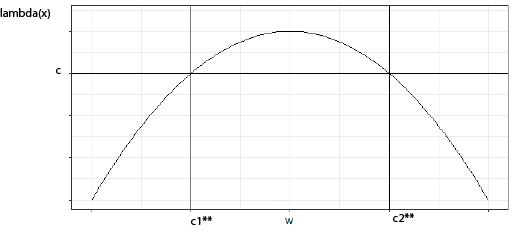
\includegraphics[scale=.8]{rcode/wplot.png}\\
\begin{multline*}\\
w=\dfrac{m}{m+n\left(\dfrac{m\sum y_i}{n\sum y_i}\right)}=\dfrac{\sum x_i}{\sum x_i+\sum y_i} \Rightarrow 0\leq w\leq 1\\
\lm(x,y) \text{ is a quadratic function of } w\\
\text{w is a monotone decreasing function of r}\\
R=\{\lm(x,y)\leq c \} \lra \{w<c_1^* \} \text{ or } \{w>c_2^*\}\\
\lra \{r<c_1^{**}\} \text{ or } \{r>c_2^{**}\}\\
X_i\sim Exp(\mu_1)=Gamma(1,\mu_1)\\
\sum X_i\sim Gamma(m,\mu_1) \Rightarrow 2\sum X_i/\mu_1 \sim Gamma(m,2)=\chi^2_{2m}\\
2\sum Y_i/\mu_2\sim \chi^2_{2n}\\
\dfrac{2\sum X_i/\mu_1/2m}{2\sum Y_i/\mu_2/2n}=\dfrac{n\sum X_i}{m\sum Y_i}\dfrac{\mu_2}{\mu_1}=\dfrac{\Bx \mu_2}{\By \mu_1}\sim F_{2m,2n}\\
\al_1=P(\dfrac{\By}{\Bx}<c_1^*|H_0)=P(\dfrac{\mu_1\By}{\mu_2\Bx}<\dfrac{c_1^*\mu_1}{\mu_2}|H_0)\\
\dfrac{\mu_1\By}{\mu_2\Bx}\sim F_{2n,2m} \quad \dfrac{c_1^*\mu_1}{\mu_2}=c_1^* \text{ (since  } \mu_1=\mu_2 \text{ under } H_0)\\
c_1^*=F_{2n,2m,\al_1}\\
\al_2=P(\dfrac{\By}{\Bx}>c_2^*|H_0)=P(\dfrac{\mu_1\By}{\mu_2\Bx}>\dfrac{c_2^*\mu_1}{\mu_2}|H_0)\\
c_2^*=F_{2n,2m,1-\al_2}\\
\end{multline*}

	\item 
\begin{multline*}\\
\psi=\mu_2/\mu_1\\
\dfrac{\psi \Bx}{\By}=\dfrac{\mu_2 \Bx}{\mu_1\By}\sim F_{2m,2n}\perp \mu_1,\mu_2 \ (\perp \psi)\\
\text{Thus } \dfrac{\psi \Bx}{\By} \text{ is a pivotal quantity}\\
\text{Exact 95\% CI for } \psi:\\
1-\al=P(F_{2m,2n,\al_1}<\dfrac{\psi \Bx}{\By}<F_{2m,2n,1-\al_2})\\
\text{95\% CI}=P(\dfrac{\By}{\Bx}F_{2m,2n,\al_1}<\psi<\dfrac{\By}{\Bx}F_{2m,2n,1-\al_2})\\
\end{multline*}

\end{enumerate}


\end{flushleft}
\end{document}
